%%%%%%%%%%%%%%%%%%%%%%%%%%%%%%%%%%%%%%%%%%%%%%%%%%%%%%%%%%%%%%%%%%%%%%%%
%                                                                      %
%     File: Thesis_Appendix.tex                                        %
%     Tex Master: Thesis.tex                                           %
%                                                                      %
%     Author: Andre C. Marta                                           %
%     Last modified : 21 Jan 2011                                      %
%                                                                      %
%%%%%%%%%%%%%%%%%%%%%%%%%%%%%%%%%%%%%%%%%%%%%%%%%%%%%%%%%%%%%%%%%%%%%%%%

\chapter{User Survey}
\label{chapter:appendixVectors}

We asked some people to answer a survey and we got 30 answers that helped us understand photography related habits and user wishes, and compiled them in this appendix.

\section{User characterization}

Our survey started by asking the respondents to describe themselves and their libraries.


\subsubsection{Kind of Photographer} % (fold)
\label{ssub:subsubsection_name}


\begin{wrapfigure}{r}{0.3\textwidth}
	\vspace{-20pt}
	\begin{center}
		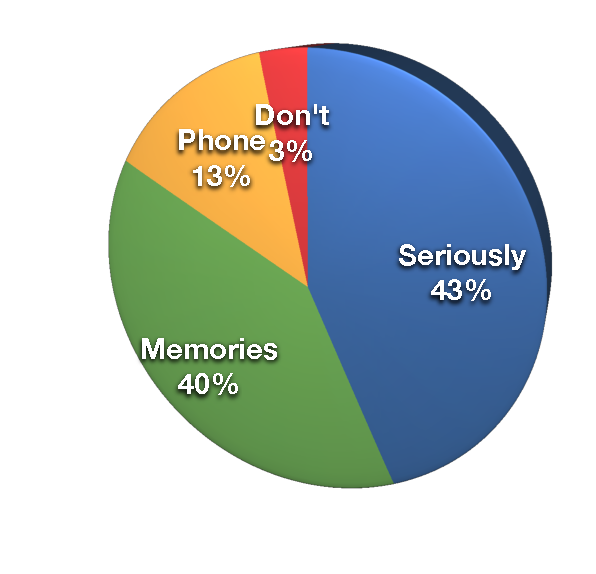
\includegraphics[width=\linewidth]{Figures/survey/desc}
	\end{center}
	\vspace{-20pt}
	\caption{Kinds of photographers.}
	\vspace{-5pt}
	\label{fig:us:desc}
\end{wrapfigure}

We asked the respondents what of the following options described them the best:

\begin{myitemize}
	\item I'm a \textbf{professional} photographer.
	\item I like to take photography \textbf{seriously} but I'm no professional.
	\item I like to take pictures just to keep as \textbf{memories}, but I'm not a photo-geek.
	\item I only use my camera \textbf{phone} for fun.
	\item I \textbf{don't} take pictures.
\end{myitemize}

As we can see on \fig{us:desc}, most respondents like photography and take photos, being mostly people who take photos for memories and people who are really into photography but are not professionals.

% subsubsection subsubsection_name (end)





\subsubsection{Storage of digital photos} % (fold)
\label{ssub:storage_of_digital_photos}
The second question was a check to verify if the respondents stored digital photos in their computers. The questionnaire would end if they said no. Fortunately, everyone said yes.
% subsubsection storage_of_digital_photos (end)





\section{Characterization of Photo Library} % (fold)
\label{sec:characterization_of_photo_library}

\begin{wrapfigure}{r}{0.5\textwidth}
	\vspace{-20pt}
	\begin{center}
		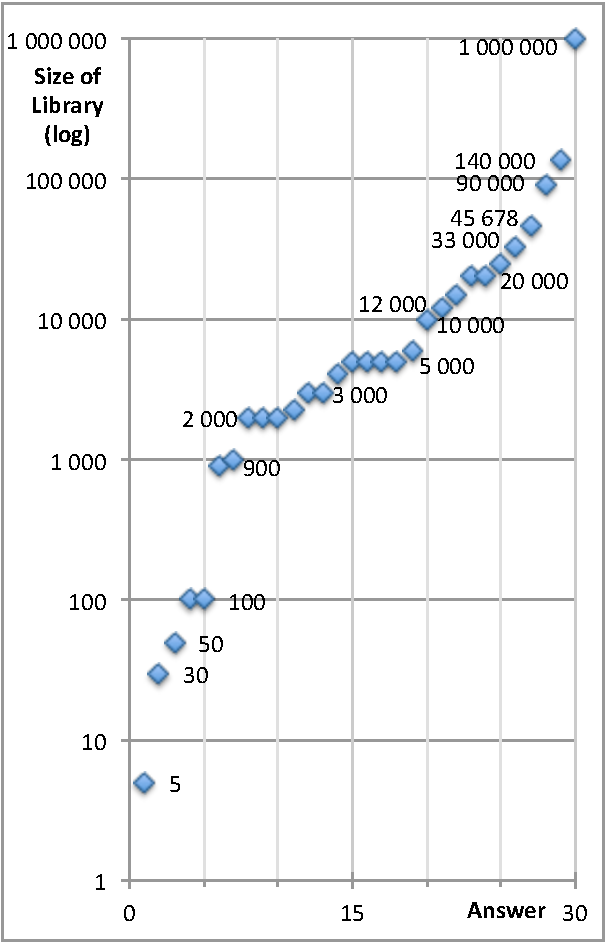
\includegraphics[width=\linewidth]{Figures/survey/libsize}
	\end{center}
	\vspace{-20pt}
	\caption{Library Size}
	\vspace{-70pt}
	\label{fig:us:desc}
\end{wrapfigure}

We then inquired about their photo libraries.
\vspace{\baselineskip}

\subsubsection{Library size} % (fold)
\label{ssub:library_size}

To start the survey about the library, we inquired how large was the respondents photo library.

We made this an open question, because we wanted to obtain real values from the users and not just limiting to a number of options that hardly represent anything. The answers for this question can be seen on \fig{us:desc}.

We were surprised by the values we got, going from 5 up to a million photos.

Almost half of the answers are between the 1 \nolinebreak 000 and the 10 000 values, having two thirds of the results falling between 0 and 10 000. We also found the median value of the answers, which is 5 \nolinebreak 000.

% subsubsection library_size (end)


\vspace{3\baselineskip}

\begin{wrapfigure}{r}{0.3\textwidth}
	\vspace{-20pt}
	\begin{center}
		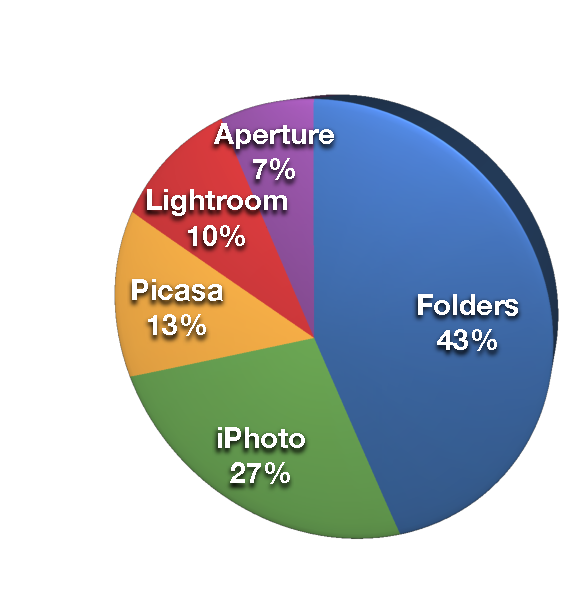
\includegraphics[width=\linewidth]{Figures/survey/sw}
	\end{center}
	\vspace{-20pt}
	\caption{Software used}
	\vspace{-5pt}
	\label{fig:us:desc}
\end{wrapfigure}

\subsubsection{Usage of Software} % (fold)
\label{ssub:usage_of_software}

We then questioned about what software applications did people use to help them organize their collections. Almost half admitted they only used folders for their organization, while the other 17 people used some kind of software.

Going through each software applications, we can see that 40\% use an entry-level software (iPhoto and Picasa) while 17\% prefer more Pro-level systems.

We tried to correlate the size of the collections with the software used but we realized that we probably don't have enough data for some of those softwares and that users might not have their entire collection inside the application, therefore defeating the correlation.

% subsubsection usage_of_software (end)

\pagebreak


\subsubsection{Systematic Organization} % (fold)
\label{ssub:systematic_organization}

\begin{wrapfigure}{r}{0.25\textwidth}
	\vspace{-20pt}
	\begin{center}
		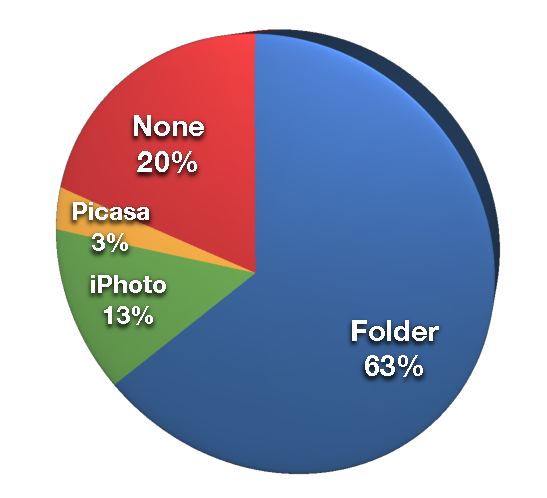
\includegraphics[width=\linewidth]{Figures/survey/organization}
	\end{center}
	\vspace{-20pt}
	\caption{Systematic organization in folders, in an application or no organization.}
	\vspace{-5pt}
	\label{fig:us:org}
\end{wrapfigure}

The question ``Do you have a systematic way to keep your photos organized?'' is meant to understand if people keep a system for their library, either on folders of inside an application.

Since most of the applications in the last question rely on folder organization, is no surprise that having a system in place for keeping things organized in folders is the clear winner of this question. Five people answered that they have this system inside an application and correlating this question with the previous one we found another expected aspect: only entry-level software is used to keep everything tidy, without touching folders, more exactly four people say they use iPhoto and one says Picasa is his/her choice.

In contrast, 20\% of the respondents claimed not having a way to organize their collections. The median of the number of photos of this group of people is 1050, the lowest, when compared to the other groups, the ones who use applications and the ones who rely on folders, both with 5000 of median.

% subsubsection systematic_organization (end)



\subsubsection{Photos in Close Sequence} % (fold)
\label{ssub:photos_in_close_sequence}

\begin{wrapfigure}{r}{0.25\textwidth}
	\vspace{-50pt}
	\begin{center}
		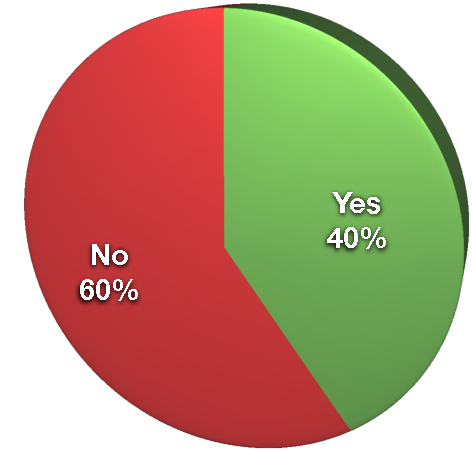
\includegraphics[width=\linewidth]{Figures/survey/close-seq}
	\end{center}
	\vspace{-20pt}
	\caption{Users that take photos in close sequence.}
	\vspace{-5pt}
	\label{fig:us:close-seq}
\end{wrapfigure}


% subsubsection photos_in_close_sequence (end)

The following question was intended to see how many users take photos in close sequence, e.g., bursts, panoramas, bracketing or time lapses, where the photographer ends up with many photos in a few seconds.

As we can see on \fig{us:close-seq}, 40\% of the respondents said they do take photos in close sequence. We also saw that this group has a median value of library size of 8000, whereas the other group stays on the 2150 images. In fact, of the total 13 enthusiasts, 11 of them answered yes on this question, followed by someone who claims only to take photos for memories.



\subsubsection{Preferred Features} % (fold)
\label{ssub:preferred_features}

\begin{wrapfigure}{r}{0.45\textwidth}
	\vspace{-50pt}
	\begin{center}
		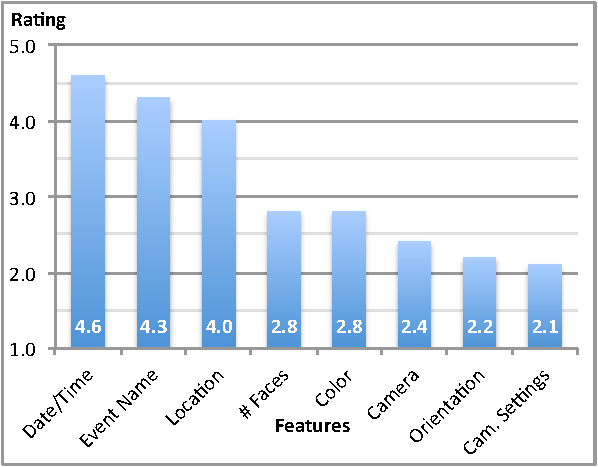
\includegraphics[width=\linewidth]{Figures/survey/features}
	\end{center}
	\vspace{-20pt}
	\caption{User rated features.}
	\vspace{-5pt}
	\label{fig:us:features}
\end{wrapfigure}

We had some ideas of what we would like to see extracted from the images and exposed to the user via our application and we asked for people's opinion on this survey and the results can be seen on \fig{us:features}.

While we weren't surprised by the favorites\linebreak Date/Time, Event and Location, we did expect\linebreak some higher ratings for number of faces and colors. Orientation and camera settings got the ratings we did expect.

% subsubsection preferred_features (end)



\subsubsection{Suggestions of Features} % (fold)
\label{ssub:suggestions_of_features}

To conclude the survey, we asked what other features they would like to see extracted from images.

\begin{itemize}

	\item The most common request, with about four different people requesting it, is people recognition. This allows photos to be tagged with the names of people in the photo and not just how many faces there are on the photo.


	\item Someone asked that, from a set of similar photos (exemplified with friend group photos), pick the one that, e.g., is more clear, has a better color, more smiles, more open eyes.


	\item Metadata was requested by three people, e.g., EXIF metadata, tags, format (RAW/JPEG), if the photo is the original or the edited version, the number of duplicates, the location on disk.


	\item One person asked for identification of wether the photo was taken during the day or the night.


	\item Another person was interested in having information about objects, buildings or animals.
\end{itemize}

\vspace{\baselineskip}

With this we concluded our survey.
% subsubsection suggestions_of_features (end)













% section characterization_of_photo_library (end)



\cleardoublepage

